\section{Effiziente Datenstrukturen für räumliche Positionen}

\todo{proofread and declutter whole section}
\todo{subsubsections}
Um große Simulationsräume mit vielen Millionen Atomen verwalten zu können, ist es offensichtlich nicht sinnvoll, alle Atome in einer Liste halten zu wollen.
Statt dessen muss man verfügbare Datenstrukturen auf ihre Leistung hinsichtlich der notwendigen Operationen betrachten.
Diese Operationen werden durch die Erfassung und Manipulation atomarer Positionen notwendig:

\begin{itemize}
\item Konstruktion \\
Der Aufbau des Simulationsraumes aus dem Substrat. Da nur einmalig durchgeführt, steht der Zeitaufwand im Hintergrund. Wichtiger ist der erwartete Speicherverbrauch.
\item Hinzufügen \\
Das Einfügen eines neuen Atomes in die Datenstruktur. Im Idealfall werden Atome in konstanter Zeit \BigO{1}) hinzugefügt.
\item Aktualisierung \\
Die Verschiebung von Atomen oder Gruppen von Atomen. Idealerweise ist konstante Zeit \BigO{m} für $m$ Atome möglich.
\item Ortssuche \\
Die Suche eines oder mehrerer Atome im Umkreis eines beliebigen Punktes. \BigO{\log{n}} oder besser ist notwendig, da diese Operation neben der Nachbarschaftssuche am häufigsten ausgeführt wird.
\item Nachbarschaftssuche \\
Die Suche nach allen Atomen im Umkreis eines anderen Atomes. Algorithmisch meist identisch zur Ortssuche, jedoch am häufigsten benutzt.
\item Oberflächensuche \\
Speziell für Wachstums- und Oberflächenprozesse muss die Oberfläche entlang einer Geraden ermittelt werden.
\end{itemize}

\subsection{Globale Atomlisten}

Der naive Ansatz ist die Speicherung aller Atome in einer globalen Liste.
Konstruktion, Hinzufügen und Aktualisierung (entsprechend \BigO{n}, \BigO{1} und \BigO{1}) weisen zwar optimale Laufzeiten auf, die anderen Operationen benötigen dagegen Worst-Case-Zeit:
Sowohl Nachbarschaftssuche als auch Ortssuche laufen in \BigO{n}.
Kombiniert mit der Suche der Oberfläche (\BigO{n}, vernachlässigt aber viele Atome) beziehungsweise der durch sie notwendigen Ereignisvalidierung summiert sich die Komplexität für eine KMC-Ereigniserstellung auf \BigO{n^2}, was allerdings verschiedene Nachbarschafts-Überprüfungen nicht mit einschließt.
Auf einer Oberfläche der Größe 400 nm$^2$ bräuchte die Erstellung eines einzigen KMC-Ereignisses auf dem Testsystem ca. 20 Sekunden, wodurch ein KMC-Schritt mit einigen tausend Ereignissen praktisch nicht durchführbar ist.

Auch Molekulardynamik-Bibliotheken kämpfen mit diesem Problem.
Um dort den Such- und Rechenaufwand bei Kraftfeldern mit Cutoff-Reichweite zu verringern, werden entweder Nachbarschaftslisten oder Binning genutzt, welches in einem folgenden Abschnitt diskutiert wird.
\textbf{Nachbarschaftslisten} referenzieren für jedes Atom alle Atome innerhalb seines Cutoff-Radius' inklusive Toleranz.
Dadurch werden Kraftberechnungen nur mit potentiell relevanten Atomen durchgeführt, allerdings müssen die Listen in regelmäßigen Intervallen aktualisiert werden, wobei jedes Mal eine \BigO{n^2}-Operation durchgeführt werden muss.
Diese Methode ist sinnvoll für mittelgroße Systeme, in denen jedes Atom in einem beschränkten Bereich wandert, stößt aber bei großen Systemen mit teilweise festen Atompositionen an seine Grenzen.

Allgemein lässt sich mit Listen von Atomen keine große Struktur in praktikabler Zeit behandeln, was an der Vielzahl nichtrelevanter Atome bei grundlegenden Operationen liegt.

\subsection{Binning oder Räumliche Datenstrukturen?}

\todo[inline]{insert content here}

\begin{figure}[bhpt]
  \captionsetup[subfigure]{singlelinecheck=false}{
    \def\subfigwidth{0.23\textwidth}
    \def\svgwidth{\textwidth}
    \begin{subfigure}[t]{\subfigwidth}
      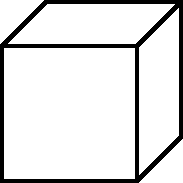
\includegraphics[width=\textwidth]{datastructures-a}
      \subcaption{Gesamter Raum (Atomlisten)}
      \label{fig:datastructures-a}
    \end{subfigure}
    \hfill
    \begin{subfigure}[t]{\subfigwidth}
      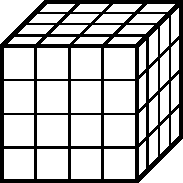
\includegraphics[width=\textwidth]{datastructures-b}
      \subcaption{Lineare Bins (k-d-Arrays)}
      \label{fig:datastructures-a}
    \end{subfigure}
    \hfill
    \begin{subfigure}[t]{\subfigwidth}
      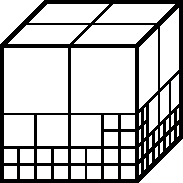
\includegraphics[width=\textwidth]{datastructures-c}
      \subcaption{Octree}
      \label{fig:datastructures-a}
    \end{subfigure}
    \hfill
    \begin{subfigure}[t]{\subfigwidth}
      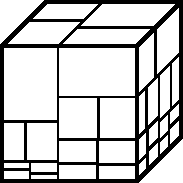
\includegraphics[width=\textwidth]{datastructures-d}
      \subcaption{k-d-Baum}
      \label{fig:datastructures-a}
    \end{subfigure}
  }
  \caption{Übersicht über räumliche Datenstrukturen}
  \label{fig:datastructures}
\end{figure}

Einerseits lässt sich der Raum in kleinere Einheiten (Zellen) unterteilen, in die dann die Atome eingefügt werden.
Somit ließe sich die Komplexität der Operation auf einen konstanten Faktor sowie die Komplexität der Suche nach der relevanten Zelle aufteilen.
Als Beispiele sind einfache mehrdimensionale Arrays sowie Octrees gegeben.

Andererseits stehen eigenständige Datenstrukturen zur Verfügung, die hinsichtlich einiger der Operationen optimiert wurden und inzwischen Standardwerkzeuge in verschiedenen Disziplinen geworden sind.
Beispiele sind hier der k-d-Baum sowie die Anwendung der Delaunay-Triangulation.

\subsection{Array-Binning}

Binning hat gemein, dass man den Raum in ausreichend große Zellen unterteilt und ihnen die darin enthaltenen Atome zuordnet.
Bei Verschiebung eines Atomes über die Grenzen seiner Zelle muss das Atom entsprechend in die benachbarte Zelle überführt werden.
Die einfachste Implementierung sieht in 3 Raumdimensionen ein dreidimensionales Array von Zellen vor.

``Linear'' bezieht sich hierbei sowohl auf die Speicherkomplexität im Verhältnis zur Anzahl der Zellen, andererseits auf die Zugriffszeiten bei Suchoperationen. Beliebiger Zugriff ist hierbei hingegen in konstanter Zeit möglich.
Orts- und Nachbarschaftssuchen geschehen in \BigO{n/N} mit $N$ Zellen für realistische Systeme, Aktualisieren und Hinzufügen geschehen in \BigO{m}.
Das Hauptproblem dieser Methode ist die potentiell große Anzahl leerer Zellen, die einerseits Speicher verbraucht, andererseits bei Oberflächensuchen zu übermäßig vielen Abfragen führt oder separate Buchhaltung benötigt (Beispiel: Heightmap).
Somit sind eigentlich zweidimensionale Oberflächenprobleme in drei Dimensionen nur kubischem Speicheraufwand möglich.

\subsection{Octree-Binning}

\begin{figure}[tbhp]
  \centering
  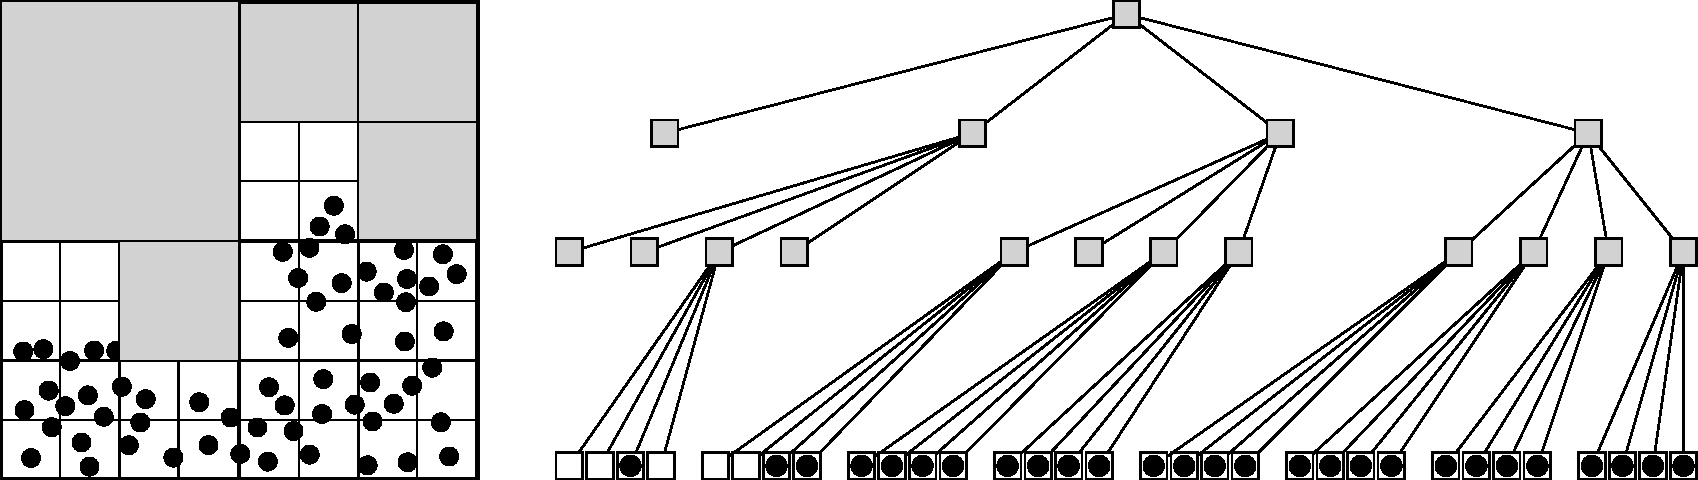
\includegraphics[width=\textwidth]{octree}
  \caption[Octree]{Octree}
  \todo[inline]{Beschreibung}
  \label{fig:octree}
\end{figure}

Ein Octree ist eine rekursive Datenstruktur, welche ebenfalls den gesamten Raum in Zellen unterteilt, dabei allerdings auf dynamische Speicherzuweisung zurückgreift und somit leere Zellen zu vermeiden versucht:
Der gesamte Raum wird als ein einziger Quader dargestellt, welchen man bei Bedarf in 8 gleiche Quader halber Breite unterteilt.
Dies geschieht rekursiv bis zur gewünschten Auflösung, bei der man die Zellen referenziert und entsprechende Atome einfügt.
8 Quader können auch wieder zu ihrer Stammzelle zusammengefügt werden, um nach getaner Arbeit den Speicher freizugeben.

Durch dieses Allokierungsschema werden die allokierten Zellen auf den interessanten Bereich beschränkt, während leeren Bereichen die Information über fehlende Atome beigelegt wird, ohne Zellen anzulegen.
Damit lassen sich Oberflächenprobleme mit zweidimensionalem Speicheraufwand betrachten, wobei im Gegenzug der Zugriff auf eine beliebige Zelle auf \BigO{\log{N}} für $N$ Zellen steigt.
Dieser Komplexität folgen auch alle Operationen, mit Ausnahme der Oberflächensuche.
Diese wird durch den Octree stark vereinfacht, da man einen großen Bereich leerer Zellen mit einem Mal überspringen kann:

Angenommen, die obere Hälfte eines großen Simulationsraumes ist komplett frei von Atomen, was nach dem Laden des Substrates typischerweise der Fall ist.
Für eine Prüfung einer Zelle muss man diese jedes Mal aus dem Arbeitsspeicher in den CPU-Cache laden, was bei modernen CPUs um die tausend CPU-Takte ($\approx$1ms) kosten kann.
Sucht man nun in einem 3d-Array die Oberfläche in Z-Richtung, so prüft man an einer xy-Position jede Zelle auf die Zahl ihrer Atome.
Dafür muss man jede Zelle aus dem Speicher laden, obwohl die Prüfung vor allem am Anfang der Simulation fehl schlägt.
Bei einem Octree hingegen wäre die obere Hälfte in vier leere Zellen zerlegt, die in der xy-Ebene nebeneinander liegen.
Somit muss man nur eine einzige Superzelle prüfen, die aufgrund der Häufigkeit der Prüfungen bereits im CPU-Cache liegt und in der Regel nicht mehr geladen werden muss.
Das Ergebnis ist ein Speedup um viele Größenordnungen bei einer der häufigsten Operationen.
Durch aktives Caching lässt sich das \BigO{\log{N}}-Verhalten dämpfen, was den Octree zur passendsten Binning-Datenstruktur erhebt.

\subsection{k-d-Baum}

\begin{figure}[bthp]
  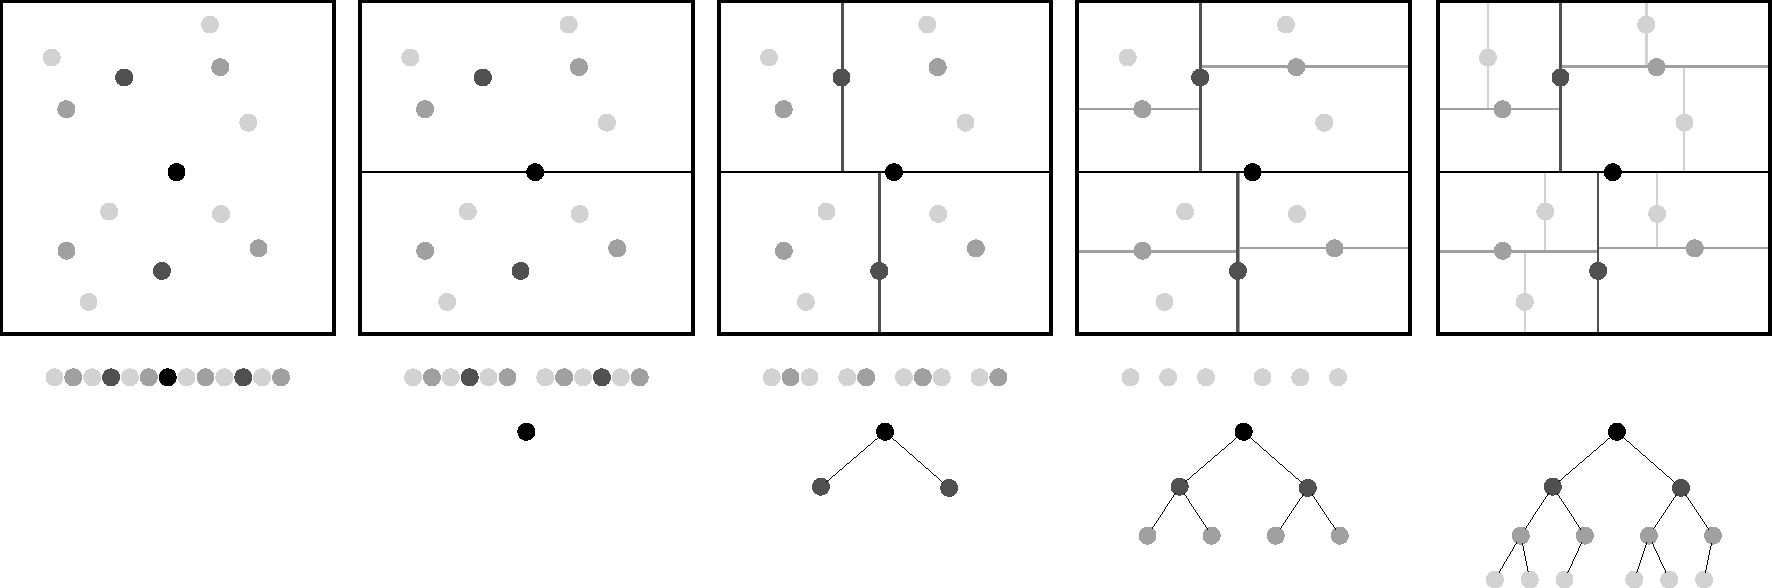
\includegraphics[width=\textwidth]{kdtree-tree}
  \caption[Konstruktion eines k-d-Baumes]{Konstruktion eines k-d-Baumes\todo[inline]{mehr Bildunterschrift}}
  \label{fig:kdtree}
\end{figure}

Wie beim Binning wird auch beim k-d-Baum (k-dimensionaler Baum) der Raum in einzelne Zellen unterteilt.
Anders als beim Binning hält jede Zelle nur ein einziges Atom.
Die Konstruktion geschieht folgendermaßen:
\begin{algorithm}
  \begin{algorithmic}
    \IF{N$\ge$1}
    \STATE Sortiere die Atome in Richtung der aktuellen Dimension (beginne mit x)
    \STATE Wähle Atom $\lfloor N/2 \rfloor$
    \STATE Teile Raum an $pos[d]_{\lfloor N/2 \rfloor}$ in zwei Zellen. Verteile die Atome auf beide Zellen.
    \STATE Wähle zyklisch die nächste Dimension
    \STATE Für beide Zellen: Gehe zu 1.
    \STATE kehre zurück
    \ENDIF
  \end{algorithmic}
  \caption[Konstruktion eines k-d-Baumes]{Konstruktion eines k-d-Baumes}
  \label{algo:kdtree-construction}
\end{algorithm}

Diese rekursive Definition erstellt aus Listen von Atomen k-d-Bäume, bei denen jeder Knoten jeweils ein Atom hält.

K-d-Bäume haben somit ein ausgezeichnetes Speicherverhalten von \BigO{n} mit recht guten Such-, Einfügungs-, Entfernungs- und Aktualisierungszeiten von \BigO{\log{n}} für realistische Systeme und niedrige Dimensionszahl.
Da es sich einfach um einen mehrdimensionalen Suchbaum handelt, lassen sich Nachbarschaftsbeziehungen ebenfalls in \BigO{\log{n}} auflösen, was für die vorliegenden Probleme immer noch hervorragend ist.
Auch bei k-d-Bäumen ist die Suche nach einer eventuellen Oberfläche jedoch nicht so einfach.
Zwar lässt sich leicht feststellen, dass nahe der Oberflächen größere Zellen existieren, jedoch lassen sich somit keine Eindellungen erfassen.
Dafür müsste man wiederum eine Vielzahl von Atomen separat auslesen und vergleichen, wofür man für jede Prüfung implizit eine Delaunay-Triangulation aufbauen muss.
Somit eignen sich k-d-Bäume zwar für die meisten Operationen hervorragend, jedoch erfüllen sie nicht alle notwendigen Voraussetzungen.
Am wichtigsten ist jedoch, dass ein k-d-Baum allgemein keine periodischen Räume unterstützt.
Zwar gibt es dafür wiederum Variationen, jedoch verlieren diese dann einige der Sucheigenschaften.

\subsection{Delaunay-Triangulation}

\begin{figure}[bhpt]
  \centering
  \def\svgwidth{\textwidth}
  \input{img/delaunay.pdf_tex}
  \caption[Delaunay-Konstruktion]{Delaunay-Konstruktion}
  \label{fig:delaunay}
\end{figure}

Während bei den bisher vorgestellten Partitionsmethoden der Raum in k-dimensionale Quader geteilt wurde, basieren Triangulationen auf k-dimensionalen Simplexen, deren Eckpunkte die gespeicherte Punktmenge bilden.
Der Zentrale Vertreter ist die Delaunay-Triangulation, die für eine Menge von Punkten folgende Eigenschaften aufweist:

\begin{itemize}
\item Jeder Punkt ist ein Eckpunkt mindestens eines Simplexes
\item Simplexe überschneiden sich nicht
\item Innerhalb des Umkreises eines Simplexes befinden sich keine weiteren Punkte
\item Die Vereinigung aller Simplexe ergibt die konvexe Hülle
\item Ein Punkt teilt sich mit seinem nächsten Nachbarn mindestens einen Simplex \\
$\Leftrightarrow$ Nächstnachbargraph $\subset$ Delaunay-Triangulation
%% \item Die Delaunay-Triangulation und das Voronoi-Diagramm über die selben Punkte sind dual\\
%% $\Rightarrow$ Allgemeine Nachbarschaftssuche ist \BigO{n\log n}
\end{itemize}

Eine Delaunay-Triangulation lässt sich aus einer Punktmenge in \BigO{n\log n}\todo{Referenz} ausführen, wofür eine Vielzahl an Algorithmen zur Verfügung stehen. \todo{Referenz}
Diesen liegt das Delaunay-Kriterium zu Grunde:
Der Umkreis eines Simplex' enthält nur seine eigenen Eckpunkte.
Ist dieses Kriterium bei zwei benachbarten Simplexen nicht gegeben, lässt sich per \textbf{Flip-Algorithmus} (Abbildung \ref{fig:delaunay-flip}) wieder eine Delaunay-Triangulation herstellen.
Dazu entfernt man die gemeinsame Kante bzw. Fläche der beiden betroffenen Simplexe und fügt zwischen den übrigen Punkten eine neue Grenze so ein, dass das Delaunay-Kriterium erfüllt ist.
Die dabei neu entstehenden Simplexe müssen nun mit ihren jeweiligen Nachbarn auf das Delaunay-Kriterium überprüft werden, wobei die neuen Simplexe als Bestandteil der Delaunay-Triangulation garantiert sind.\todo{Referenz}

\begin{figure}[bhpt]
  \captionsetup[subfigure]{singlelinecheck=false}{
    \def\subfigwidth{0.23\textwidth}
    \def\svgwidth{\textwidth}
    \begin{subfigure}[t]{\subfigwidth}
      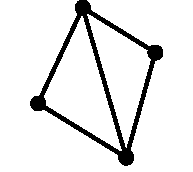
\includegraphics[width=\textwidth]{delaunay-flip-a}
      \subcaption{Ausgangstriangulation}
      \label{fig:delaunay-flip-a}
    \end{subfigure}
    \hfill
    \begin{subfigure}[t]{\subfigwidth}
      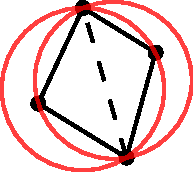
\includegraphics[width=\textwidth]{delaunay-flip-b}
      \subcaption{Vereinigung invalider Simplexe}
      \label{fig:delaunay-flip-b}
    \end{subfigure}
    \hfill
    \begin{subfigure}[t]{\subfigwidth}
      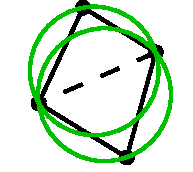
\includegraphics[width=\textwidth]{delaunay-flip-c}
      \subcaption{Aufteilung in neue valide Simplexe}
      \label{fig:delaunay-flip-c}
    \end{subfigure}
    \hfill
    \begin{subfigure}[t]{\subfigwidth}
      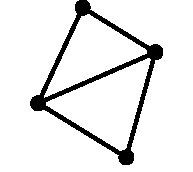
\includegraphics[width=\textwidth]{delaunay-flip-d}
      \subcaption{Ergebnis}
      \label{fig:delaunay-flip-d}
    \end{subfigure}
  }
  \caption{Flip Algorithmus zur Aktualisierung einer Delaunay-Triangulation}
  \label{fig:delaunay-flip}
\end{figure}

\todo{Laufzeit Flipping?}

Für die Nachbarschaftssuche eines Referenzpunktes werden die raumfüllenden Eigenschaften der Triangulation relevant.
Der notwendigerweise konvexe, sonst aber beliebige Suchbereich um den Referenzpunkt wird von Simplexen überdeckt, die in direkter oder indirekter Nachbarschaft des Punktes liegen.
Somit teilen sich alle Punkte innerhalb des Suchbereiches eine Kante eines Simplexes mit einem anderen Punkt im Suchbereich.
Man muss nun einfach alle Kanten der Triangulation absuchen, bis man Punkte außerhalb des Suchbereiches findet.
Ein möglicher Algorithmus kann folgendermaßen aussehen:

\begin{algorithm}
  \centering
  \begin{algorithmic}
    \STATE Result = \{\}
    \STATE Queue = \{ P$_0$ : P$_0 \in$ Volume \}
    \WHILE{Queue $\neq \emptyset$}
    \STATE Sei P $\in$ Queue
    \STATE Queue = Queue $\setminus$ \{ P \}
    \IF{P $\in$ Volume}
    \STATE Result = Result $\cap$ \{ P \}
    \STATE Queue $\cap$ (Neighbors(P) $\setminus$ Result)
    \ENDIF
    \ENDWHILE
  \end{algorithmic}
  \caption[Nachbarschaftssuche auf einer Delaunay-Triangulation]{Nachbarschaftssuche auf einer Delaunay-Triangulation}
  \label{algo:delaunay-neighbors}
\end{algorithm}

\todo[inline]{continue here}

Dabei wird ausgenutzt, dass die Delaunay-Triangulation raumfüllend ist.
Somit werden nur Atome und Primitive untersucht, die Bestandteil des Suchraumes sind, weshalb diese Suche lokal und somit schnell bleibt.

Um die Position einzelner Punkte zu aktualisieren, arbeitet man üblicherweise mit Flip-Algorithmen, wie in Abbildung \ref{fig:delaunay-flip} dargestellt.

Hinsichtlich der Oberflächensuche wird allerdings eine andere Eigenschaft offensichtlich:
Die Alpha-Oberfläche ist ein Subgraph der Delaunay-Triangulation.
Vereinfacht ausgedrückt ist die Alpha-Form einer Punktmenge ihre ``ungefähre Form'', wie man sie wahrnehmen würde.
Oft zieht man auch Parallelen zum ``Einpacken in Plastikfolie mit Luftabpumpen''.
Die eigentliche Definition beinhaltet folgende Idee:

\begin{figure}[bhpt]
  \centering
  \captionsetup[subfigure]{singlelinecheck=false}{
    \def\subwidth{0.3\textwidth}
    \def\svgwidth{\textwidth}
    \begin{subfigure}[t]{\subwidth}
      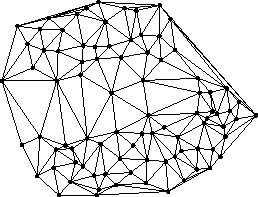
\includegraphics[width=\textwidth]{delaunay-alpha-a}
      \subcaption{Delaunay Triangulation}
      \label{fig:delaunay-alpha-a}
    \end{subfigure}
    \hfill
    \begin{subfigure}[t]{\subwidth}
      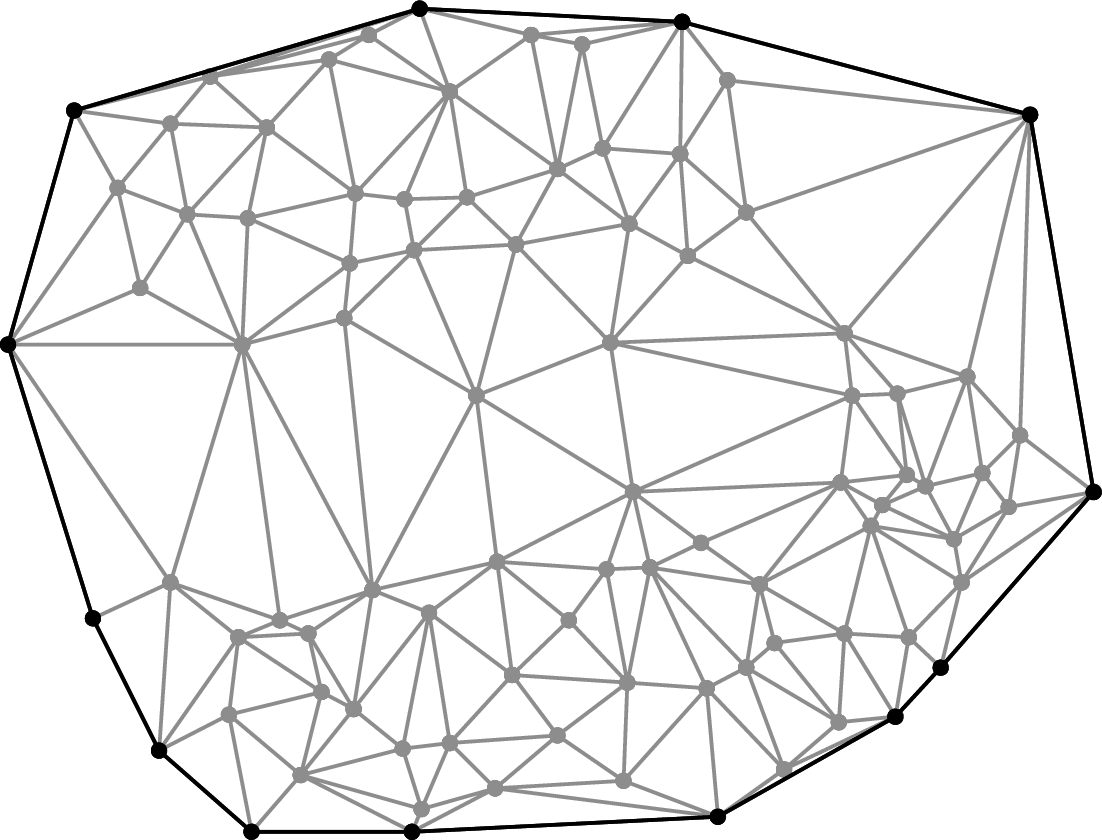
\includegraphics[width=\textwidth]{delaunay-alpha-b}
      \subcaption{Konvexe Hülle: Kanten mit nur einem Simplex}
      \label{fig:delaunay-alpha-b}
    \end{subfigure}
    \hfill
    \begin{subfigure}[t]{\subwidth}
      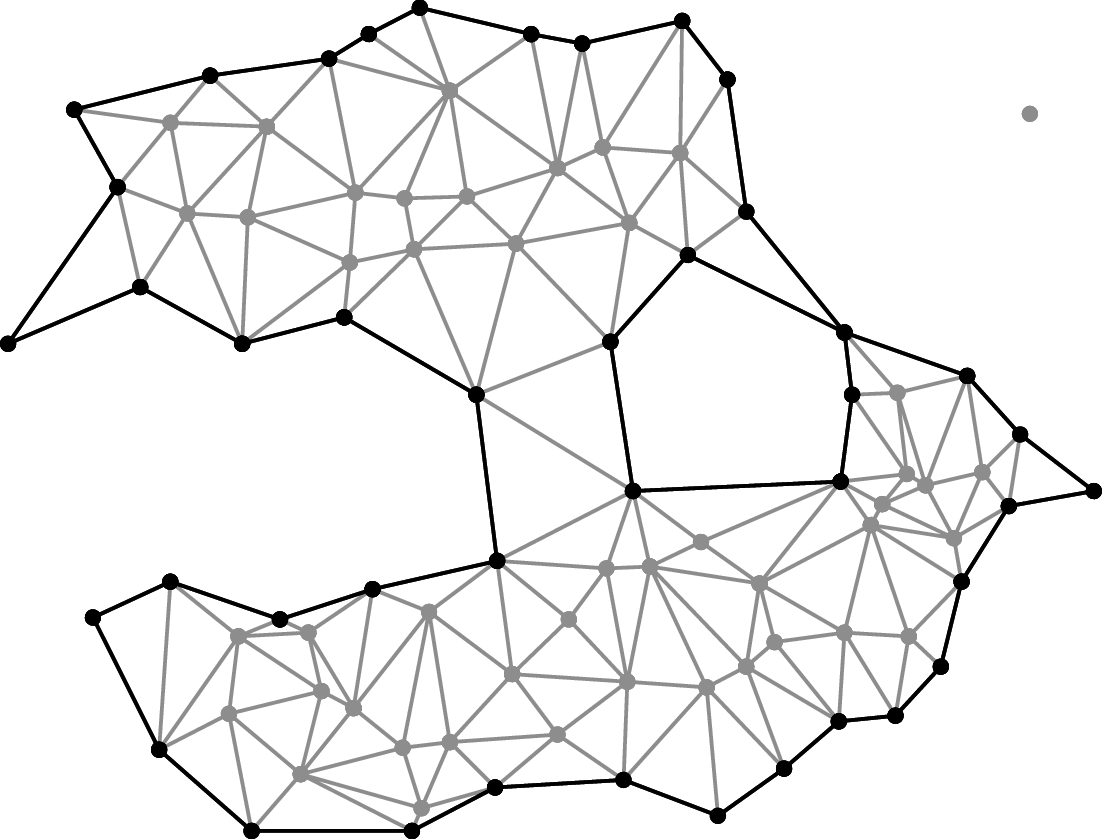
\includegraphics[width=\textwidth]{delaunay-alpha-c}
      \subcaption{Alpha-Form: Hülle nach Entfernung von Simplexen mit $\text{Umkreis} > \alpha$}
      \label{fig:delaunay-alpha-c}
    \end{subfigure}
  }
  \caption{Konstruktion einer Alpha-Form}
  \label{fig:delaunay-alpha}
\end{figure}

Entfernt man alle Delaunay-Primitive, deren Umkreisradius oberhalb eines Grenzwertes $\alpha$ liegt, und bildet dann die Vereinigung aller verbleibenden Primitive sowie etwaiger frei gewordener Punkte, so erhält man die Alphaform.
Für $\alpha = \infty$ erhält man somit die konvexe Hülle.
Für endliche Werte von $\alpha$ hingegen werden auch konkave Bereiche in der Oberfläche betrachtet.
Wählt man $\alpha$ jedoch unterhalb des kleinsten Abstandes der Atome, so erfasst man zwangsläufig auch Atome im Inneren der Struktur, wodurch die Idee der allgemeinen Oberfläche wieder verloren geht.

Verwaltet man nun parallel zur Delaunay-Triangulation eine Liste der theoretisch durch den $alpha$-Algorithmus entfernten Primitive, so hat man die Oberfläche der gesamten Struktur charakterisiert, ohne nennenswerten Mehraufwand treiben zu müssen.
Durch Kenntnis dieser Oberfläche ließen sich nun CVD-Prozesse auch an spitzen Strukturen betrachten, ohne dem Wachstum die Charakteristika der räumlichen Darstellung aufzuzwingen.

Bisher ist es jedoch bei theoretischen Betrachtungen dieser Delaunay-basierten Methoden geblieben.
Hinsichtlich allgemeiner Oberflächensimulationen ließe sich diese Methode der Delaunay-Triangulationen perspektivisch in Parsivald einpflegen.
